% Options for packages loaded elsewhere
% Options for packages loaded elsewhere
\PassOptionsToPackage{unicode}{hyperref}
\PassOptionsToPackage{hyphens}{url}
\PassOptionsToPackage{dvipsnames,svgnames,x11names}{xcolor}
%
\documentclass[
]{standalone}
\usepackage{xcolor}
\usepackage{amsmath,amssymb}
\setcounter{secnumdepth}{-\maxdimen} % remove section numbering
\usepackage{iftex}
\ifPDFTeX
  \usepackage[T1]{fontenc}
  \usepackage[utf8]{inputenc}
  \usepackage{textcomp} % provide euro and other symbols
\else % if luatex or xetex
  \usepackage{unicode-math} % this also loads fontspec
  \defaultfontfeatures{Scale=MatchLowercase}
  \defaultfontfeatures[\rmfamily]{Ligatures=TeX,Scale=1}
\fi
\usepackage{lmodern}
\ifPDFTeX\else
  % xetex/luatex font selection
\fi
% Use upquote if available, for straight quotes in verbatim environments
\IfFileExists{upquote.sty}{\usepackage{upquote}}{}
\IfFileExists{microtype.sty}{% use microtype if available
  \usepackage[]{microtype}
  \UseMicrotypeSet[protrusion]{basicmath} % disable protrusion for tt fonts
}{}
\makeatletter
\@ifundefined{KOMAClassName}{% if non-KOMA class
  \IfFileExists{parskip.sty}{%
    \usepackage{parskip}
  }{% else
    \setlength{\parindent}{0pt}
    \setlength{\parskip}{6pt plus 2pt minus 1pt}}
}{% if KOMA class
  \KOMAoptions{parskip=half}}
\makeatother
% Make \paragraph and \subparagraph free-standing
\makeatletter
\ifx\paragraph\undefined\else
  \let\oldparagraph\paragraph
  \renewcommand{\paragraph}{
    \@ifstar
      \xxxParagraphStar
      \xxxParagraphNoStar
  }
  \newcommand{\xxxParagraphStar}[1]{\oldparagraph*{#1}\mbox{}}
  \newcommand{\xxxParagraphNoStar}[1]{\oldparagraph{#1}\mbox{}}
\fi
\ifx\subparagraph\undefined\else
  \let\oldsubparagraph\subparagraph
  \renewcommand{\subparagraph}{
    \@ifstar
      \xxxSubParagraphStar
      \xxxSubParagraphNoStar
  }
  \newcommand{\xxxSubParagraphStar}[1]{\oldsubparagraph*{#1}\mbox{}}
  \newcommand{\xxxSubParagraphNoStar}[1]{\oldsubparagraph{#1}\mbox{}}
\fi
\makeatother


\usepackage{longtable,booktabs,array}
\usepackage{calc} % for calculating minipage widths
% Correct order of tables after \paragraph or \subparagraph
\usepackage{etoolbox}
\makeatletter
\patchcmd\longtable{\par}{\if@noskipsec\mbox{}\fi\par}{}{}
\makeatother
% Allow footnotes in longtable head/foot
\IfFileExists{footnotehyper.sty}{\usepackage{footnotehyper}}{\usepackage{footnote}}
\makesavenoteenv{longtable}
\usepackage{graphicx}
\makeatletter
\newsavebox\pandoc@box
\newcommand*\pandocbounded[1]{% scales image to fit in text height/width
  \sbox\pandoc@box{#1}%
  \Gscale@div\@tempa{\textheight}{\dimexpr\ht\pandoc@box+\dp\pandoc@box\relax}%
  \Gscale@div\@tempb{\linewidth}{\wd\pandoc@box}%
  \ifdim\@tempb\p@<\@tempa\p@\let\@tempa\@tempb\fi% select the smaller of both
  \ifdim\@tempa\p@<\p@\scalebox{\@tempa}{\usebox\pandoc@box}%
  \else\usebox{\pandoc@box}%
  \fi%
}
% Set default figure placement to htbp
\def\fps@figure{htbp}
\makeatother





\setlength{\emergencystretch}{3em} % prevent overfull lines

\providecommand{\tightlist}{%
  \setlength{\itemsep}{0pt}\setlength{\parskip}{0pt}}



 


% preamble.tex
\usepackage{tikz}
\usepackage{xcolor}
\usepackage{multicol}
\usetikzlibrary{positioning,arrows.meta,fit}
\tikzset{>=Stealth}

\tikzstyle{arrow} = [thick,->,>=stealth]

\definecolor{exblue}{HTML}{005377}
\definecolor{exgreen}{HTML}{06A77D}

\definecolor{highlight}{HTML}{A3C87B}
\tikzstyle{role} = [rectangle, rounded corners, minimum width=1cm, minimum height=1cm,text centered, draw=black]

% Farger
\definecolor{cTop}{RGB}{230,170,160}
\definecolor{cInvest}{RGB}{32,75,111}
\definecolor{cFinance}{RGB}{146,185,221}
\definecolor{cPayout}{RGB}{0,128,128}
\makeatletter
\@ifpackageloaded{caption}{}{\usepackage{caption}}
\AtBeginDocument{%
\ifdefined\contentsname
  \renewcommand*\contentsname{Table of contents}
\else
  \newcommand\contentsname{Table of contents}
\fi
\ifdefined\listfigurename
  \renewcommand*\listfigurename{List of Figures}
\else
  \newcommand\listfigurename{List of Figures}
\fi
\ifdefined\listtablename
  \renewcommand*\listtablename{List of Tables}
\else
  \newcommand\listtablename{List of Tables}
\fi
\ifdefined\figurename
  \renewcommand*\figurename{Figure}
\else
  \newcommand\figurename{Figure}
\fi
\ifdefined\tablename
  \renewcommand*\tablename{Table}
\else
  \newcommand\tablename{Table}
\fi
}
\@ifpackageloaded{float}{}{\usepackage{float}}
\floatstyle{ruled}
\@ifundefined{c@chapter}{\newfloat{codelisting}{h}{lop}}{\newfloat{codelisting}{h}{lop}[chapter]}
\floatname{codelisting}{Listing}
\newcommand*\listoflistings{\listof{codelisting}{List of Listings}}
\makeatother
\makeatletter
\makeatother
\makeatletter
\@ifpackageloaded{caption}{}{\usepackage{caption}}
\@ifpackageloaded{subcaption}{}{\usepackage{subcaption}}
\makeatother
\usepackage{bookmark}
\IfFileExists{xurl.sty}{\usepackage{xurl}}{} % add URL line breaks if available
\urlstyle{same}
\hypersetup{
  colorlinks=true,
  linkcolor={blue},
  filecolor={Maroon},
  citecolor={Blue},
  urlcolor={Blue},
  pdfcreator={LaTeX via pandoc}}


\author{}
\date{}
\begin{document}


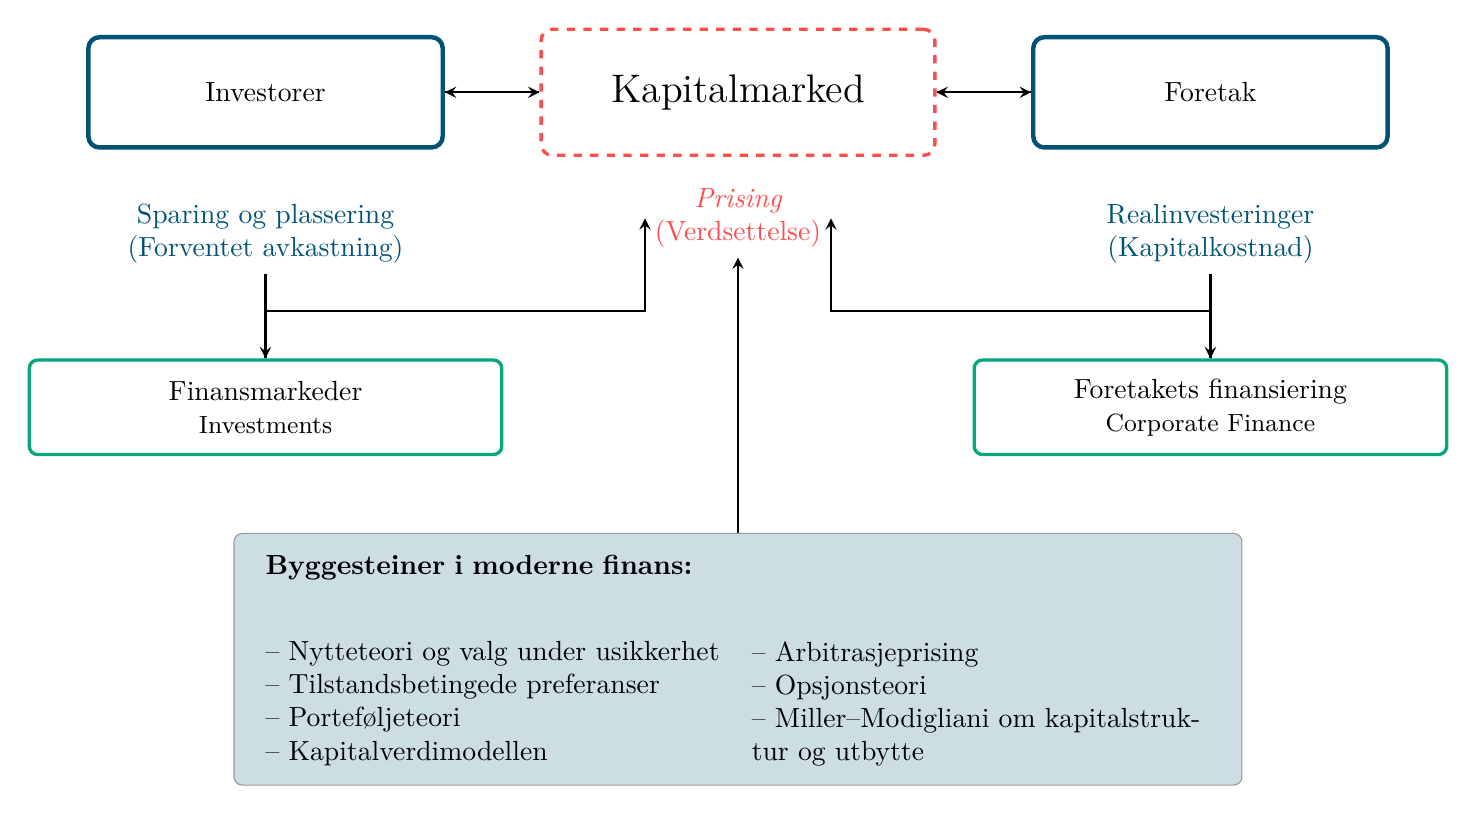
\begin{tikzpicture}
    % Ramme og grunnposisjoner
\begin{scope}[x=1cm,y=1cm]
  % Hovednoder
  \node[role, minimum width=4.5cm, minimum height=1.4cm, draw=exblue, ultra thick, fill=white] (investors) at (-6,0) {Investorer};
  \node[role, minimum width=5.0cm, minimum height=1.6cm, draw=red!70, very thick, dashed, fill=white] (market) at (0,0) {\Large Kapitalmarked};
  \node[role, minimum width=4.5cm, minimum height=1.4cm, draw=exblue, ultra thick, fill=white] (firms) at (6,0) {Foretak};

  % Tokoblede piler mellom hovednoder
  \draw[arrow] (investors) -- (market);
  \draw[arrow] (market) -- (investors);
  \draw[arrow] (firms) -- (market);
  \draw[arrow] (market) -- (firms);

  % Undertekster venstre og høyre
  \node[align=center, text=exblue] (leftsub)  at (-6,-1.8) {Sparing og plassering\\(Forventet avkastning)};
  \node[align=center, text=exblue] (rightsub) at ( 6,-1.8) {Realinvesteringer\\(Kapitalkostnad)};

  % Prising under markedet
  \node[align=center, text=red!70] (pricing) at (0,-1.6) {\it Prising\\(Verdsettelse)};

  % Fagområder nederst
  \node[rectangle, rounded corners=3pt, minimum width=6.0cm, minimum height=1.2cm, draw=exgreen, very thick, fill=white, align=center] (investments) at (-6,-4.0) {Finansmarkeder\\\small Investments};
  \node[rectangle, rounded corners=3pt, minimum width=6.0cm, minimum height=1.2cm, draw=exgreen, very thick, fill=white, align=center] (corpfin)     at ( 6,-4.0) {Foretakets finansiering\\\small Corporate Finance};

  % Piler fra undertekster ned til fagbokser
  \draw[arrow] (leftsub)  -- (investments);
  \draw[arrow] (rightsub) -- (corpfin);

  % Piler opp til prising fra fagbokser
  \draw[arrow] (investments.north) -- ++(0,0.6) -| (pricing.west);
  \draw[arrow] (corpfin.north)     -- ++(0,0.6) -| (pricing.east);

  % Fundament for faget nederst i midten
\node[rectangle, rounded corners=3pt, draw=black!40, fill=exblue!20,
      minimum width=12.8cm, text width=12cm, align=left, inner sep=8pt]
      (foundation) at (0,-7.2)
  {
    \textbf{Byggesteiner i moderne finans:}\\[4pt]
    \begin{multicols}{2}
      -- Nytteteori og valg under usikkerhet\\
      -- Tilstandsbetingede preferanser\\
      -- Porteføljeteori\\
      -- Kapitalverdimodellen \\
      -- Arbitrasjeprising\\
      -- Opsjonsteori\\
      -- Miller--Modigliani om kapitalstruktur og utbytte
    \end{multicols}
  };

  % Diskrete piler fra fundament til midt
  \draw[arrow] (foundation.north) -- (pricing.south);
\end{scope}

\end{tikzpicture}




\end{document}
